% Provenance (never printed): see sources/outline_sources.md (Year 2: Hadean, Archean and
% Proterozoic; early crust and greenstone belts; the oxygenation of the atmosphere; snowball
% Earth). Eons and eras from the ICS chart; greenstone belts, TTG and cratons after Cawood and
% others (2018) and Smithies and others (2019); komatiite liquidus after Sossi and O'Neill (2016),
% Pierru and others (2022) and Asimow (2022); the Archean air and the GOE after Catling and Zahnle
% (2020) and Luo and others (2016); the boring billion after Lyons and others (2021); snowball
% Earth after Hoffman and others (2017). The energy-balance model, the komatiite line and the CO2
% build-up from figdata/bachelor-2/precambrian.py; exercise and problem values in the Book 4
% scratch calculator calc/ch18.py.
\chapter{La Terre précambrienne}\label{ch:b2:precambrian-earth}

Les premiers fossiles à coquille apparaissent dans des roches vieilles d'environ 540 millions
d'années. Tout ce qui précède, depuis la naissance de la Terre il y a \qty{4567}{Ma}, est le Précambrien~: sept huitièmes
de l'histoire de la planète. Pendant ce temps, la Terre a bâti les noyaux de ses continents et rempli son air d'oxygène,
et elle s'est figée au moins deux fois, des pôles à l'équateur, avec des calottes glaciaires atteignant la mer
sous les tropiques. Ce chapitre lit ces quatre milliards d'années dans les roches qui en subsistent, et
chiffre trois de leurs énigmes~: pourquoi les laves les plus anciennes étaient si chaudes, comment une planète gelée peut
dégeler, et comment la jeune Terre est restée tiède sous un Soleil faible.
% ledger: ics:base.Hadean, ics:base.Phanerozoic, hoffman17:cryochrons

\begin{recall}
\textbf{Acquis des volumes scolaires}~: l'âge de la Terre~; les éons de l'échelle des temps géologiques~;
la loi de luminosité du jeune Soleil et le \omterm{def:b2:precambrian-earth:faint-sun}{paradoxe du Soleil jeune}~; l'atmosphère primitive~;
les stromatolithes, les \omterm{def:b2:precambrian-earth:bif}{formations de fer rubanées}, la \omterm{def:b2:precambrian-earth:goe}{Grande Oxydation} et les grès rouges~; les \omterm{def:b2:precambrian-earth:craton}{cratons}~;
la chaleur radiogénique du passé. \textbf{Acquis du volume de première année}~: le zircon et ses âges U--Pb,
sa température de fermeture~; la production de chaleur radiogénique des quatre isotopes~; le rayonnement
infrarouge sortant et l'insolation moyenne globale $S_0/4$~; les unités chronostratigraphiques.
\textbf{Acquis des chapitres précédents}~: la \omterm{def:b2:mantle-melting:tp}{température potentielle du manteau} et l'adiabate
(\cref{ch:b2:mantle-melting})~; le liquidus et la \omterm{def:b2:magmatic-differentiation:crystallisation}{cristallisation fractionnée} de l'olivine
(\cref{ch:b2:magmatic-differentiation})~; les types de granites (\cref{ch:b2:crustal-melting})~;
les \omterm{def:b2:wilson-cycle:supercontinent}{supercontinents} (\cref{ch:b2:wilson-cycle}). L'oxydation et la réduction relèvent des livres de chimie,
et les premiers eucaryotes et la photosynthèse des livres de biologie.
\end{recall}

\section{Trois éons avant les fossiles}\label{sec:b2:precambrian-earth:eons}

\begin{definition}[Hadéen, Archéen, Protérozoïque]\label{def:b2:precambrian-earth:eons}
Le temps antérieur au Phanérozoïque se divise en trois éons. L'\emph{Hadéen}\index{Hadéen}
s'étend de la formation de la Terre, il y a \qty{4567}{Ma}, jusqu'à $4031 \pm \qty{3}{Ma}$~; le
\emph{Archéen}\index{Archéen} va de $4031$ à \qty{2500}{Ma}~; le
\emph{Protérozoïque}\index{Protérozoïque} va de 2500 à \qty{538.8}{Ma}, base du Cambrien.
Ensemble, on les appelle de façon informelle le Précambrien.
\end{definition}
% ledger: ics:base.Hadean, ics:base.Archean, ics:base.Proterozoic, ics:base.Phanerozoic

L'\omterm{def:b2:precambrian-earth:eons}{Archéen} se divise en quatre ères, l'Éoarchéen (4031 à \qty{3600}{Ma}), le Paléoarchéen (3600
à 3200), le Mésoarchéen (3200 à 2800) et le Néoarchéen (2800 à 2500)~; le \omterm{def:b2:precambrian-earth:eons}{Protérozoïque} en trois,
le Paléoprotérozoïque (2500 à \qty{1600}{Ma}), le Mésoprotérozoïque (1600 à 1000) et
le Néoprotérozoïque (1000 à 538.8). Deux périodes néoprotérozoïques comptent ci-dessous~: le Cryogénien, de 720 à
\qty{635}{Ma}, et l'Édiacarien, de 635 à \qty{538.8}{Ma}.
% ledger: ics4:archean-eras, ics4:proterozoic-eras

\begin{omfigure}
\centering
% ledger: ics:base.Hadean, ics:base.Archean, ics:base.Proterozoic, ics:base.Phanerozoic, ics4:archean-eras, ics4:proterozoic-eras, wilde01:4404, bowring99:acasta, cz20:impacts, allwood06:spc, cawood18:transition, gumsley17:goe, luo16:goe, hoffman17:earlier, earle:bif, lyons21:boring, hoffman17:ages, asimow22:komatiite
\begin{tikzpicture}[x=-3.4cm, y=1cm, font=\scriptsize]
% eons
\fill[icsHadean] (4.567,0) rectangle (4.031,0.5);
\fill[icsArchean] (4.031,0) rectangle (2.5,0.5);
\fill[icsProterozoic] (2.5,0) rectangle (0.5388,0.5);
\fill[icsPhanerozoic] (0.5388,0) rectangle (0,0.5);
\node[text=white] at (4.299,0.25) {Hadéen};
\node[text=white] at (3.27,0.25) {Archéen};
\node[text=white] at (1.52,0.25) {Protérozoïque};
\node at (0.27,0.25) {Phan.};
% eras
\foreach \a/\b/\c in {4.031/3.6/35, 3.6/3.2/55, 3.2/2.8/35, 2.8/2.5/55}
  \fill[icsArchean!\c] (\a,-0.45) rectangle (\b,0);
\foreach \a/\b/\c in {2.5/1.6/35, 1.6/1.0/55, 1.0/0.5388/35}
  \fill[icsProterozoic!\c] (\a,-0.45) rectangle (\b,0);
\foreach \x/\l in {3.8155/Éo, 3.4/Paléo, 3.0/Méso, 2.65/Néo, 2.05/Paléo, 1.3/Méso, 0.769/Néo}
  \node at (\x,-0.225) {\l};
% axis
\draw (4.6,-0.6) -- (0,-0.6);
\foreach \t in {0,0.5,...,4.5} {
  \draw (\t,-0.6) -- (\t,-0.7);
  \node[anchor=north] at (\t,-0.7) {\pgfmathprintnumber[fixed, precision=1]{\t}};
}
\node[anchor=north, font=\small] at (2.3,-1.05) {temps avant le présent (milliards d'années)};
% row A
\fill[omDef] (4.404,0.85) circle (2pt);
\node[anchor=west, text=omDef] at (4.404,0.85) {zircon le plus ancien};
\fill[omMeth] (3.43,0.85) circle (2pt);
\node[anchor=west, text=omMeth] at (3.43,0.85) {premiers stromatolithes};
\draw[red!60!black, line width=3pt] (2.4,0.85) -- (1.8,0.85);
\node[anchor=west, text=red!60!black] at (1.8,0.85) {formations de fer rubanées};
% row B
\fill[omDef] (4.03,1.5) circle (2pt);
\node[anchor=west, text=omDef] at (4.03,1.5) {roches les plus anciennes};
\draw[black!70, line width=3pt] (3.2,1.5) -- (2.5,1.5);
\node[anchor=south, text=black!80] at (2.85,1.6) {changement de style tectonique};
\draw[omProp, line width=3pt] (1.8,1.5) -- (0.8,1.5);
\node[anchor=south, text=omProp] at (1.3,1.6) {«~milliard ennuyeux~»};
% row C
\draw[black!60, line width=2pt, densely dashed] (4.2,2.25) -- (3.5,2.25);
\node[anchor=south, text=black!70] at (3.85,2.35) {grand bombardement tardif~? (débattu)};
\draw[omThm, line width=3pt] (2.43,2.25) -- (2.06,2.25);
\node[anchor=west, text=omThm] at (2.06,2.25) {Grande Oxydation};
% row D
\fill[blue!60!black] (2.4,3.0) circle (2pt);
\node[anchor=east, text=blue!60!black] at (2.4,3.0) {première Terre boule de neige};
\fill[omThm] (0.8,3.0) circle (2pt);
\node[anchor=east, text=omThm] at (0.8,3.0) {seconde montée de l'oxygène};
% row E
\fill[orange!80!black] (1.9,3.7) circle (2pt);
\node[anchor=east, text=orange!80!black] at (1.9,3.7) {dernières komatiites courantes};
\draw[blue!60!black, line width=3pt] (0.717,3.7) -- (0.635,3.7);
\node[anchor=east, text=blue!60!black] at (0.717,3.7) {Terres boules de neige du Cryogénien};
% row F
\fill[omMeth] (0.57,4.4) circle (2pt);
\node[anchor=east, text=omMeth] at (0.57,4.4) {premiers grands fossiles (Édiacarien)};
\end{tikzpicture}
\par\smallskip{\small Le Précambrien en une ligne. Les éons et, en teintes plus claires, leurs ères
(Éo-, Paléo-, Méso- et Néoarchéen~; Paléo-, Méso- et Néoprotérozoïque) sont ceux de la Charte
chronostratigraphique internationale~; les événements sont placés aux âges cités dans le texte.
Les «~dernières \omterm{def:b2:precambrian-earth:greenstone}{komatiites} courantes~» sont celles qui ne sont pas appauvries en aluminium~; il en existe de plus jeunes et de plus rares.}
\end{omfigure}

\subsection*{L'Hadéen~: des minéraux sans roches}

Aucune roche de l'\omterm{def:b2:precambrian-earth:eons}{Hadéen} ne subsiste, seulement des minéraux. Le plus ancien est un grain de zircon
des Jack Hills, en Australie-Occidentale, de $4404 \pm \qty{8}{Ma}$, arraché à une roche plus ancienne
et déposé dans un conglomérat vieux d'environ trois milliards d'années. Sa composition, et celle de ses voisins,
a été interprétée par ses découvreurs comme la preuve qu'une croûte de type continental et de l'eau liquide
existaient déjà il y a \qty{4.4}{Ga}, environ 160 millions d'années après la formation de la Terre. Les plus
anciennes roches datées, les gneiss d'Acasta, dans le nord-ouest du Canada, ont entre 4.00 et
\qty{4.03}{Ga}, proches de la base de l'\omterm{def:b2:precambrian-earth:eons}{Archéen}.
% ledger: wilde01:4404, wilde01:zircon, uw14:jack-hills, bowring99:acasta

La jeune Terre a été frappée par de grands corps, comme l'expose au
\cref{ch:b2:planet-formation-meteorites}. Le dernier impact assez puissant pour vaporiser
tout l'océan remonterait à environ \qty{4.3}{Ga}. Un «~grand bombardement tardif~»,
une rafale d'impacts entre environ 4.2--4.0 et \qty{3.5}{Ga} déduite des âges des roches lunaires
et des chocs enregistrés dans les \omterm{def:b2:planet-formation-meteorites:fall-find}{météorites}, a été proposé~; beaucoup contestent qu'il s'agisse
d'un événement distinct, et, dans les deux cas, il n'aurait probablement pas stérilisé la Terre.
% ledger: cz20:impacts

\section{La croûte archéenne}\label{sec:b2:precambrian-earth:archean}

\subsection*{Ceintures de roches vertes et komatiites}

La croûte archéenne qui subsiste est faite de deux types de terrains juxtaposés~: de vastes massifs de gneiss granitiques gris,
riches en sodium, et des ceintures plus étroites de roches volcaniques et sédimentaires altérées.

\begin{definition}[Ceinture de roches vertes~; komatiite]\label{def:b2:precambrian-earth:greenstone}
Une \emph{ceinture de roches vertes}\index{ceinture de roches vertes} est un ensemble de roches volcaniques mafiques et ultramafiques,
avec des sédiments, métamorphisées à faible degré (le vert vient de la chlorite, de l'actinote et de
l'épidote), prises entre des massifs de granitoïdes archéens et, dans certains terrains, protérozoïques. Une
\emph{komatiite}\index{komatiite} est une lave ultramafique, bien plus riche en MgO que le basalte,
émise à l'état liquide~; son olivine forme en général de longues lames minces, la
texture \emph{spinifex}, le sommet de la coulée refroidissant vite.
\end{definition}
% ledger: cawood18:dome-keel, so16:liquidus, pierru22:komatiite

\begin{omfigure}
\centering
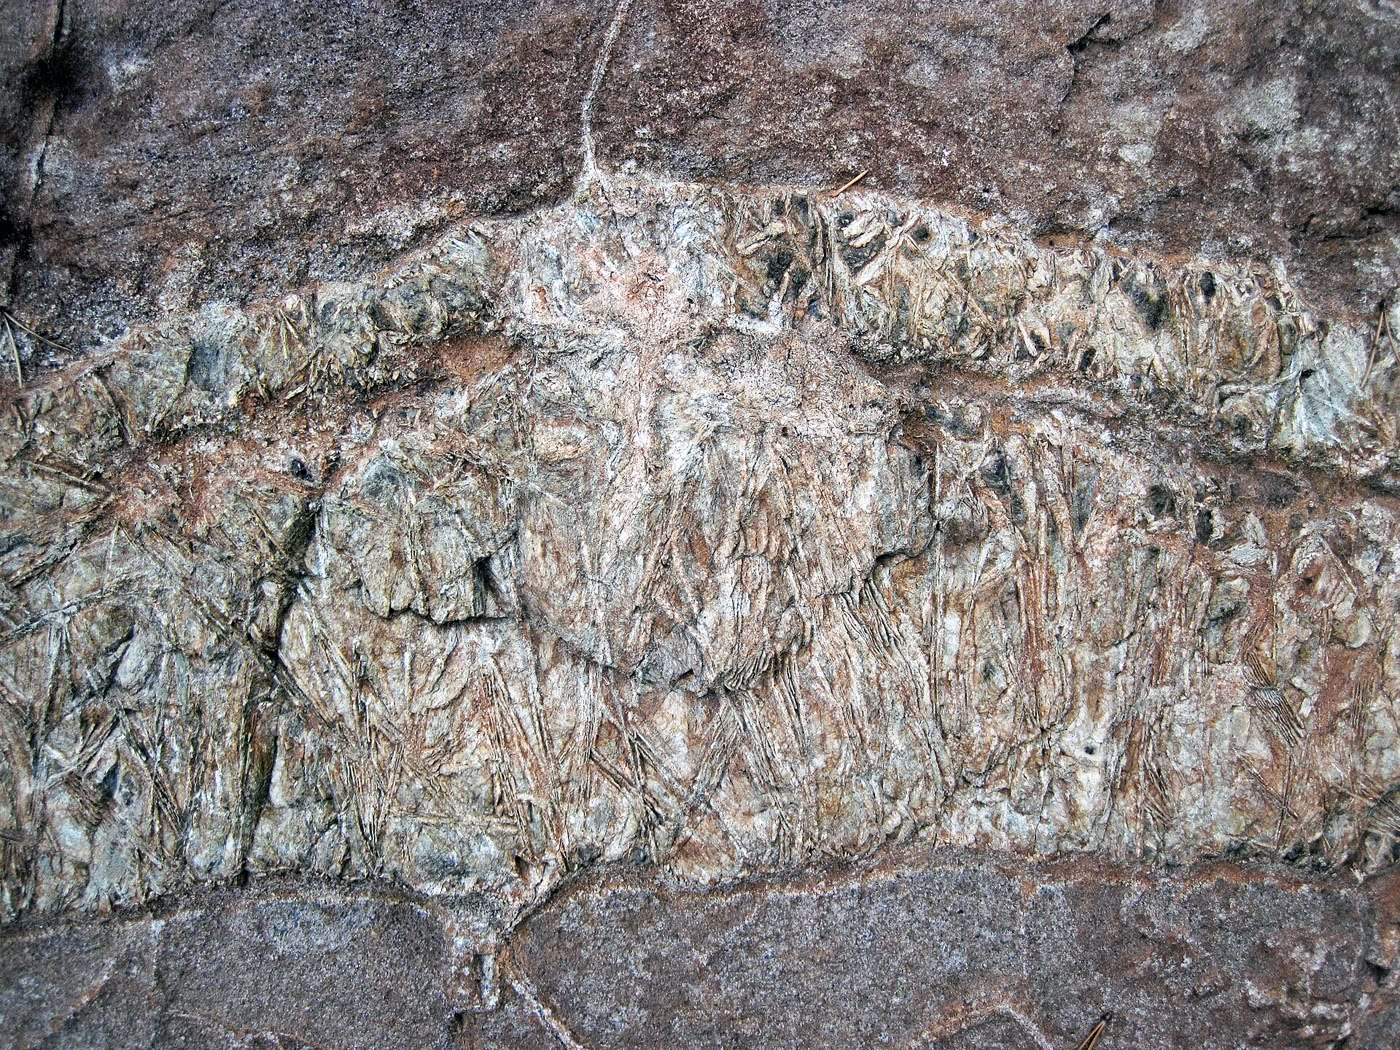
\includegraphics[width=0.66\linewidth]{images/book4/b2-18-spinifex-komatiite.jpg}
\par\smallskip{\small Texture spinifex dans une coulée de \omterm{def:b2:precambrian-earth:greenstone}{komatiite}, Pyke Hill (Ontario), partie d'une
\omterm{def:b2:precambrian-earth:greenstone}{ceinture de roches vertes} néoarchéenne vieille d'environ 2.71~milliards d'années~: des lames d'olivine, aujourd'hui altérées,
ont poussé à travers le sommet refroidi de la coulée. Photographie James St.~John, CC~BY~2.0 (Wikimedia
Commons).}
\end{omfigure}

Les \omterm{def:b2:precambrian-earth:greenstone}{komatiites} contiennent jusqu'à \qty{34}{\percent} de MgO, contre 10 à \qty{13}{\percent} dans les basaltes
primaires des dorsales actuelles, et elles sont presque cantonnées à la vieille Terre~: le type appauvri en aluminium
n'existe que dans des roches plus anciennes que \qty{2.8}{Ga}, le type non appauvri jusque vers
\qty{1.9}{Ga}, et seul un rare type enrichi en aluminium est aussi jeune que \qty{90}{Ma}. Un liquide
aussi riche en magnésium est très chaud et, comme pour les basaltes étudiés
au \cref{ch:b2:magmatic-differentiation}, le premier minéral à cristalliser est l'olivine,
dont la fraction dans le liquide fixe la température.
% ledger: pierru22:komatiite, asimow22:komatiite

\begin{proposition}[Le thermomètre à komatiites]\label{prop:b2:precambrian-earth:liquidus}
Pour un liquide en équilibre avec l'olivine à la pression atmosphérique, la température du liquidus
croît à peu près linéairement avec la teneur en MgO du liquide. Par deux expériences $(m_1, T_1)$ et
$(m_2, T_2)$,
\[
  T_{\text{liq}}(m) = T_1 + s\,(m - m_1), \qquad s = \frac{T_1 - T_2}{m_1 - m_2} .
\]
Des expériences de fusion sur deux \omterm{def:b2:precambrian-earth:greenstone}{komatiites}, $\qty{32.2}{\percent}$ de MgO à \qty{1616}{\celsius} et
$\qty{23}{\percent}$ à \qty{1450}{\celsius}, donnent $s = \qty{18.0}{\celsius}$ par point de pourcentage de
MgO.
\end{proposition}
% ledger: so16:liquidus, helz98:glass-thermometer

\begin{proof}
L'olivine est une solution solide de forstérite et de fayalite, bien plus riche en magnésium que le liquide
dont elle se forme. À mesure que le liquide refroidit, l'olivine lui prélève du magnésium, et la température à
laquelle le liquide est juste saturé en olivine baisse avec sa teneur en MgO. Les expériences montrent que, sur l'intervalle
d'une famille donnée de liquides, la baisse est presque linéaire, si bien que la droite passant par
deux expériences interpole entre elles~; $s = (1616 - 1450)/(32.2 - 23) = 166/9.2 = 18.04$.
\end{proof}

Ce coefficient n'est pas propre aux \omterm{def:b2:precambrian-earth:greenstone}{komatiites}. Des verres trempés à partir de la lave du Kilauea,
calibrés de la même façon, varient de \qty{3}{\celsius} pour \qty{0.15}{\percent} de MgO, soit
\qty{20}{\celsius} par point de pourcentage. Prolonger la droite des \omterm{def:b2:precambrian-earth:greenstone}{komatiites} jusqu'à un basalte primaire de dorsale
à \qty{12}{\percent} de MgO donne son liquidus à quelques dizaines de degrés près~: $1616 -
18.0\times20.2 \approx \qty{1252}{\celsius}$. Les liquides de \omterm{def:b2:precambrian-earth:greenstone}{komatiites} les plus chauds étaient donc
d'environ \qty{360}{\celsius} plus chauds que les liquides qui alimentent les dorsales actuelles, et la figure ci-dessous
montre la droite.
% ledger: helz98:glass-thermometer, so16:liquidus, pierru22:komatiite
% values: slope 18.043, T_morb12 1251.5, dT_kom_morb 364.5 (precambrian.py)

\begin{omfigure}
\centering
\begin{tikzpicture}
\begin{axis}[omrecord, width=0.72\linewidth, height=6cm, xmin=8, xmax=35, ymin=1150, ymax=1700,
  xlabel={MgO dans le liquide (\unit{\percent} en masse)}, ylabel={liquidus à 1 atm (\unit{\celsius})},
  xtick pos=bottom, ytick pos=left, clip=false,
  y tick label style={/pgf/number format/1000 sep={}}]
% computed in figdata/bachelor-2/precambrian.py part kom; ledger: so16:liquidus, pierru22:komatiite
\fill[omProp!15] (axis cs:10,1150) rectangle (axis cs:13,1700);
\addplot[black, line width=1.1pt] table[x=MgO, y=T] {figdata/out/bachelor-2-precambrian-kom.dat};
\addplot[only marks, mark=*, mark size=2.4pt, omThm] coordinates {(32.2,1616) (23,1450)};
\node[anchor=north west, font=\scriptsize, text=omThm] at (axis cs:32.2,1612) {Barberton};
\node[anchor=north west, font=\scriptsize, text=omThm] at (axis cs:23,1446) {Munro};
\node[anchor=south, font=\scriptsize, text=omProp, align=center] at (axis cs:11.5,1560)
  {basaltes primaires\\de dorsale};
\draw[densely dashed] (axis cs:12,1150) -- (axis cs:12,1251.5) -- (axis cs:8,1251.5);
\draw[densely dashed] (axis cs:32.2,1150) -- (axis cs:32.2,1616);
\draw[<->, omDef, thick] (axis cs:27,1251.5) -- (axis cs:27,1616);
\draw[densely dotted] (axis cs:12,1251.5) -- (axis cs:27,1251.5);
\draw[densely dotted] (axis cs:27,1616) -- (axis cs:32.2,1616);
\node[anchor=east, font=\scriptsize, text=omDef] at (axis cs:26.7,1330) {environ \qty{360}{\celsius}};
\end{axis}
\end{tikzpicture}
\par\smallskip{\small Le thermomètre à \omterm{def:b2:precambrian-earth:greenstone}{komatiites}~: la droite passant par les températures de liquidus
mesurées sur deux \omterm{def:b2:precambrian-earth:greenstone}{komatiites} (points), prolongée jusqu'aux 10 à \qty{13}{\percent} de MgO des basaltes primaires
des dorsales actuelles (bande). Le prolongement repose sur la pente voisine des liquides basaltiques.}
\end{omfigure}

Une lave plus chaude ne signifie pas un manteau plus chaud d'autant. Les \omterm{def:b2:precambrian-earth:greenstone}{komatiites} ont probablement remonté en
panaches, comme les basaltes les plus chauds d'aujourd'hui à Hawaï, où la température potentielle monte
jusqu'à environ \qty{200}{\celsius} au-dessus des $1350 \pm \qty{50}{\celsius}$ du manteau ambiant. Elles se sont
formées par de forts \omterm{def:b2:mantle-melting:fraction}{taux de fusion}, à plus grande profondeur. On pense couramment qu'elles se sont formées dans un
manteau de 200 à \qty{300}{K} plus chaud que l'actuel~; une autre hypothèse veut que les \omterm{def:b2:precambrian-earth:greenstone}{komatiites}
soient des \omterm{def:b2:magma-emplacement:magma}{magmas} humides, formés à des températures pas beaucoup plus élevées que celles du manteau environnant.
Dans les deux cas, le manteau archéen était plus chaud, et les volumes scolaires en donnaient une raison~:
il y a 3 milliards d'années, les quatre isotopes radioactifs libéraient plus de
deux fois la chaleur actuelle (\cref{exo:b2:precambrian-earth:2}).
% ledger: asimow22:komatiite, pierru22:komatiite, so16:liquidus

\subsection*{Le TTG et le motif dômes-et-quilles}

Les gneiss gris situés entre les \omterm{def:b2:precambrian-earth:greenstone}{ceintures de roches vertes} ne sont pas des granites du type que
décrit au \cref{ch:b2:crustal-melting}.

\begin{definition}[Suite tonalite--trondhjémite--granodiorite]\label{def:b2:precambrian-earth:ttg}
La \emph{suite tonalite--trondhjémite--granodiorite}\index{suite tonalite--trondhjémite--granodiorite}
(TTG) est la famille des granitoïdes riches en sodium et pauvres en potassium --- tonalites,
trondhjémites (tonalites pauvres en minéraux mafiques) et granodiorites --- qui constituent l'essentiel
de la croûte continentale archéenne. La plupart se sont formées par \omterm{def:b2:mantle-melting:melting}{fusion partielle} de croûte basaltique
hydratée.
\end{definition}
% ledger: smithies19:ttg, cawood18:ttg

Une grande partie du volume de la croûte continentale actuelle s'était formée à la fin de l'\omterm{def:b2:precambrian-earth:eons}{Archéen}, surtout
sous forme de TTG. Certains TTG portent des signatures en éléments traces longtemps lues comme une fusion à plus
de \qty{50}{km} de profondeur, une pression non atteinte dans la croûte continentale plus jeune, et ces lectures
pèsent dans le débat sur le début de la tectonique des plaques~; une étude de 2019 a soutenu que ces signatures
proviennent plutôt de liquides du manteau, et que les TTG courants se sont formés à des
profondeurs ne dépassant pas les \qty{40}{km} d'une croûte continentale ordinaire aujourd'hui. Vers la fin
de l'\omterm{def:b2:precambrian-earth:eons}{Archéen}, entre environ 3.0 et \qty{2.5}{Ga}, les granitoïdes de la plupart des \omterm{def:b2:precambrian-earth:craton}{cratons} passent des TTG
aux granites riches en potassium, signe qu'une croûte plus épaisse était de nouveau fondue.
% ledger: smithies19:ttg, cawood18:ttg

Dans l'est de la Pilbara, en Australie, au Zimbabwe et dans le sud de l'Inde, les deux terrains dessinent un
motif frappant sur la carte. Des dômes arrondis de granitoïdes sont encadrés par des quilles synclinales de roches vertes dont les couches plongent et s'éloignent des dômes. Les dômes sont
vraisemblablement montés sous forme de \omterm{def:b2:magma-emplacement:ascent}{diapirs}, la croûte granitique légère remontant à travers une épaisse pile dense de
laves qui s'étaient enfoncées entre eux. Dans la Pilbara, ce dômage a duré des centaines de millions
d'années et s'est arrêté il y a environ \qty{3.1}{Ga}, après quoi les structures deviennent linéaires,
comme celles des \omterm{def:b2:alpine-orogen:orogen}{orogènes} plus jeunes.
% ledger: cawood18:dome-keel

\begin{omfigure}
\centering
\begin{tikzpicture}[x=0.95cm, y=0.95cm, font=\scriptsize]
% schematic, after the description in cawood18:dome-keel
\fill[lith basalt] (0,0) rectangle (12,7);
\draw (0,0) rectangle (12,7);
\foreach \cx/\cy/\rx/\ry in {2.4/4.7/1.7/1.4, 7.2/5.0/2.0/1.4, 4.6/1.6/1.9/1.1, 10.0/2.0/1.4/1.3}
  \filldraw[lith granite, draw=black, thick] (\cx,\cy) ellipse ({\rx} and {\ry});
% strike and dip in the greenstone, each dipping away from the nearest dome
% (positions and strikes from the outward normals of the ellipses, computed by hand)
\foreach \px/\py/\st in {3.9/5.99/309, 0.9/5.99/231, 0.9/3.41/129, 2.4/2.88/90, 4.52/4.7/0,
    9.62/5.0/0, 8.91/6.29/305, 5.49/6.29/235, 8.91/3.71/55, 5.49/3.71/125,
    6.92/1.6/0, 4.6/3.12/270, 2.28/1.6/180, 6.24/0.53/60,
    10.0/3.72/270, 11.29/0.78/47, 8.18/2.0/180, 11.29/3.22/313}
  \pic at (\px,\py) {strikedip={\st}{}};
\node[fill=white, inner sep=1.5pt] at (2.4,4.7) {dôme TTG};
\node[fill=white, inner sep=1.5pt] at (7.2,5.0) {dôme TTG};
\node[fill=white, inner sep=1.5pt] at (4.6,1.6) {dôme TTG};
\node[fill=white, inner sep=1.5pt] at (10.0,2.0) {dôme TTG};
\node[fill=white, inner sep=1.5pt, align=center] at (7.45,2.75) {roches vertes\\quille};
\node[fill=white, inner sep=1.5pt, align=center] at (1.0,0.9) {roches vertes};
\pic at (11.4,5.6) {northarrow};
% section below
\begin{scope}[yshift=-3.3cm]
\fill[lith basalt] (0,0) -- (12,0) -- (12,2.2) -- (0,2.2) -- cycle;
\filldraw[lith granite, draw=black, thick] (0.6,0) .. controls (0.6,2.0) and (4.6,2.0) .. (4.6,0) -- cycle;
\filldraw[lith granite, draw=black, thick] (6.4,0) .. controls (6.4,2.1) and (11.0,2.1) .. (11.0,0) -- cycle;
\draw[thick] (0,0) rectangle (12,2.2);
\draw[black!70] (4.6,0.9) .. controls (5.5,0.2) .. (6.4,0.9);
\draw[black!70] (4.35,1.5) .. controls (5.5,0.6) .. (6.65,1.5);
\node[fill=white, inner sep=1.5pt] at (2.6,0.6) {TTG};
\node[fill=white, inner sep=1.5pt] at (8.7,0.6) {TTG};
\node[fill=white, inner sep=1.5pt] at (5.5,1.75) {quille};
\draw[->, thick] (2.6,1.0) -- (2.6,1.75);
\draw[->, thick] (8.7,1.05) -- (8.7,1.8);
\draw[->, thick] (5.5,1.4) -- (5.5,0.95);
\node[anchor=west] at (12.1,1.1) {coupe};
\end{scope}
\node[anchor=west] at (12.1,3.5) {carte};
\end{tikzpicture}
\par\smallskip{\small Le motif dômes-et-quilles de certains \omterm{def:b2:precambrian-earth:craton}{cratons} archéens (schéma, non à
l'échelle). Carte~: dômes de granitoïdes de la suite TTG encadrés par des roches vertes~; les symboles
direction-pendage montrent les couches des roches vertes plongeant à l'écart de chaque dôme. Coupe~: les dômes
remontent tandis que la pile dense de roches vertes s'enfonce en quilles synclinales entre eux (flèches).}
\end{omfigure}

\subsection*{Cratons}

\begin{definition}[Craton]\label{def:b2:precambrian-earth:craton}
Un \emph{craton}\index{craton} est une partie d'un continent restée tectoniquement stable
pendant plus d'un milliard d'années~: un noyau de croûte archéenne ou protérozoïque, métamorphique et
plutonique, reposant sur une racine épaisse, froide et peu dense de manteau lithosphérique qui atteint environ
\qty{250}{km} de profondeur.
\end{definition}
% ledger: tulane:cratons, fischer:lithosphere, cawood18:ttg

Les \omterm{def:b2:precambrian-earth:craton}{cratons} se sont stabilisés surtout au Mésoarchéen et au Néoarchéen, et les signes de cette
stabilité sont inscrits dans les roches~: de larges bassins sédimentaires posés dessus, comme le
supergroupe du Transvaal sur le \omterm{def:b2:precambrian-earth:craton}{craton} du Kaapvaal (environ 2640 à \qty{2055}{Ma}) et le supergroupe du Mount Bruce
sur la Pilbara (2775 à \qty{2210}{Ma})~; des essaims de \omterm{def:b2:magma-emplacement:bodies}{dykes} rectilignes qui les recoupent comme des plaques
cassantes~; et leurs racines épaisses, acquises à la fin de l'\omterm{def:b2:precambrian-earth:eons}{Archéen}. Entre 3.2 et
\qty{2.5}{Ga}, les archives montrent aussi les plus anciennes marges passives et des \omterm{def:b2:alpine-orogen:foreland}{bassins d'avant-pays}, des ceintures
de \omterm{def:b2:metamorphic-facies:metamorphism}{métamorphisme} apparié, et des indices paléomagnétiques de déplacements relatifs des \omterm{def:b2:precambrian-earth:craton}{cratons}.
Une revue de 2018 lit ces changements comme l'installation progressive de la tectonique des plaques telle qu'elle fonctionne
aujourd'hui, tout en soulignant qu'aucune observation isolée ne la prouve~; les estimations publiées de ce
début vont de l'\omterm{def:b2:precambrian-earth:eons}{Hadéen} au Néoprotérozoïque.
% ledger: cawood18:transition, cawood18:ttg, cawood18:cratons

\begin{inthefield}[Lire une ceinture de roches vertes]
Dans une \omterm{def:b2:precambrian-earth:greenstone}{ceinture de roches vertes}, la première question que se pose le géologue cartographe est dans quel sens les
roches étaient orientées à leur formation, puisque les couches sont souvent verticales ou renversées. Les laves en coussins
donnent la réponse par leurs sommets arrondis et les bases pointues qu'elles poussent dans les coussins sous-jacents~;
les lits granoclassés par leur diminution de taille vers le haut~; et les coulées de \omterm{def:b2:precambrian-earth:greenstone}{komatiite} par leur zonation, un
sommet refroidi et fracturé traversé de lames de spinifex qui croissent vers le bas, au-dessus d'une base riche
en cristaux d'olivine accumulés. Les sens de polarité relevés station par station dessinent les synclinaux des quilles.
Les zircons des tufs felsiques et du TTG des dômes donnent alors des âges U--Pb, si bien que le géologue peut savoir
quelles roches vertes sont plus anciennes que les dômes qui les traversent aujourd'hui.
\end{inthefield}
% ledger: so16:liquidus (spinifex in the top zones of flows), cawood18:dome-keel

\section{Oxygène}\label{sec:b2:precambrian-earth:oxygen}

\subsection*{Un air archéen sans oxygène}

L'atmosphère primitive des volumes scolaires était riche en azote et en dioxyde de carbone, et pauvre en oxygène.
Les indices et les modèles la bornent aujourd'hui plus étroitement. Avant \qty{2.4}{Ga}, l'oxygène en surface
était inférieur au millionième de la valeur actuelle~; le dioxyde de carbone atteignait peut-être 10 à 2500 fois
sa valeur actuelle, et le méthane 100 à \num{10000} fois. Des grains d'uraninite et de pyrite, que l'oxygène
détruit, étaient transportés par les fleuves archéens et déposés sans altération~; à \qty{2.415}{Ga},
la survie de l'uraninite détritique impose un plafond de \qty{3.2e-5}{atm} à l'oxygène. Le cycle du carbone, rappelé
plus bas, maintenait la température moyenne de surface entre environ 0 et \qty{40}{\celsius}.
% ledger: cz20:archean-air, kasting25:indicators

L'oxygène était produit~: les cyanobactéries le libèrent par photosynthèse, et des traces en apparaissent dans
certaines roches archéennes. Mais il était consommé aussi vite qu'il se formait, par les gaz volcaniques et par le fer
dissous dans la mer.
% ledger: luo16:goe, lyons21:boring

\begin{definition}[Formation de fer rubanée]\label{def:b2:precambrian-earth:bif}
Une \emph{formation de fer rubanée}\index{formation de fer rubanée} (BIF) est un sédiment chimique
fait de fines couches alternées d'oxydes de fer --- hématite, magnétite --- et de chert. Elle précipite
à partir d'eau de mer qui transporte du fer(II) dissous, lorsque ce fer s'oxyde en fer(III) insoluble~;
elle demande donc un océan profond sans oxygène, un apport de fer
et un oxydant à l'endroit où le fer se dépose.
\end{definition}
% ledger: earle:bif, holland06:stages

Les \omterm{def:b2:precambrian-earth:bif}{formations de fer rubanées} sont les plus abondantes entre 2.4 et \qty{1.8}{Ga}~; ensuite l'océan profond
ne portait plus assez de fer dissous, et elles disparaissent presque, pour revenir brièvement dans les
dépôts glaciaires du Cryogénien (ci-dessous). Ce sont un minerai de fer courant
(voir au \cref{ch:b2:ore-deposits}).
% ledger: earle:bif, hoffman17:models

\subsection*{La Grande Oxydation}

\begin{definition}[Grande Oxydation]\label{def:b2:precambrian-earth:goe}
La \emph{Grande Oxydation}\index{Grande Oxydation} (GOE) est l'intervalle, d'environ
2.4--2.3 à environ \qty{2.1}{Ga}, pendant lequel l'oxygène s'est accumulé pour la première fois
de façon durable dans l'atmosphère et dans l'océan de surface, passant de moins d'un millionième
de son niveau actuel à peut-être un dixième.
\end{definition}
% ledger: cz20:goe, cz20:archean-air, gumsley17:goe, holland06:stages

Le marqueur le plus net est une signature des isotopes du soufre. Dans les sédiments plus anciens que la GOE, les
isotopes du soufre sont triés d'une façon que seule la photochimie dans un air sans oxygène peut produire~; la signature
disparaît dès que l'oxygène arrive. Sa physique et son archive complète relèvent du volume de troisième année~;
ici, elle sert d'horloge. Dans trois carottes de forage à travers le supergroupe du Transvaal, en Afrique du Sud,
la signature disparaît à \qty{2.33}{Ga}, en 1 à \qty{10}{Ma}~: la montée elle-même a été rapide. D'autres archives
placent le début de l'événement entre 2.46 et \qty{2.43}{Ga}, au moment de la première glaciation mondiale,
et montrent que l'oxygène n'a pas augmenté régulièrement
par la suite.
% ledger: luo16:goe, farquhar00:sulfur, pk02:anoxic, gumsley17:goe

Après la GOE apparaissent les grès rouges, la pyrite et l'uraninite détritiques disparaissent des sables fluviaux,
et les sols gardent leur fer sous forme d'oxydes. Mais l'océan profond est resté anoxique pendant plus d'un milliard
d'années.
% ledger: kasting25:indicators, lyons21:boring

\subsection*{Le «~milliard ennuyeux~» et la seconde montée}

L'intervalle d'environ 1.8 à \qty{0.8}{Ga} montre si peu de changement dans les isotopes du carbone des
carbonates marins qu'on l'appelle souvent le «~milliard ennuyeux~». Son oxygène est débattu~: des estimations anciennes
donnaient de 1 à \qty{40}{\percent} du niveau actuel, les isotopes du chrome suggèrent moins de
\qty{1}{\percent}, peut-être \qty{0.1}{\percent}. L'océan profond était anoxique. Pendant cet intervalle,
les eucaryotes, comme le racontent les livres de biologie, apparaissent, se diversifient et deviennent plus nombreux. Vers \qty{800}{Ma},
de nombreux enregistrements montrent une seconde montée brutale de l'oxygène, à l'époque de progrès majeurs de la vie complexe~;
on discute encore pour savoir si l'oxygène les a déclenchés ou s'il les a suivis. De grands fossiles de l'Édiacarien
apparaissent vers \qty{570}{Ma}. Pendant ce temps, les \omterm{def:b2:wilson-cycle:supercontinent}{supercontinents} étudiés au \cref{ch:b2:wilson-cycle}
se sont assemblés puis ont éclaté~: les marges passives, signe d'un éclatement, sont abondantes vers 2100 à
\qty{1850}{Ma}, lors de l'assemblage de Nuna, puis de nouveau de 650 à \qty{500}{Ma}.
% ledger: lyons21:boring, lyons21:eukaryotes, cawood18:ttg, nance22:supercontinents

\section{De la glace jusqu'à l'équateur}\label{sec:b2:precambrian-earth:snowball}

\subsection*{La rétroaction glace--albédo}

La neige et la glace réfléchissent l'essentiel du rayonnement solaire qu'elles reçoivent, la mer libre très peu~: environ
\qty{6}{\percent} pour l'océan, de 50 à \qty{70}{\percent} pour la banquise nue, jusqu'à
\qty{90}{\percent} pour la glace couverte de neige. Une Terre qui se refroidit fait croître la glace, réfléchit davantage
de lumière solaire et se refroidit encore.
% ledger: nsidc:albedo-ice, albedo:surfaces

\begin{definition}[Rétroaction glace--albédo]\label{def:b2:precambrian-earth:ice-albedo}
La \emph{rétroaction glace--albédo}\index{rétroaction glace--albédo} est l'amplification d'une variation
de température par la variation de couverture neigeuse et glacée qu'elle provoque~: le refroidissement étend la glace, ce qui
élève l'albédo de la planète, réduit le rayonnement solaire absorbé et refroidit encore la planète~;
le réchauffement agit à l'inverse. C'est une rétroaction positive.
\end{definition}
% ledger: hoffman17:hysteresis, nsidc:albedo-ice

Ses conséquences apparaissent dans le modèle climatique le plus simple~: une planète d'une seule température $T$ et
de capacité thermique $C$ par mètre carré. Elle absorbe $\tfrac14 S(1 - a)$, où $S$ est le rayonnement solaire
à sa distance et $a$ son albédo, et elle perd le rayonnement infrarouge sortant du volume de première année, écrit
$\varepsilon\sigma T^4$~: $\varepsilon$, l'\emph{émissivité effective}, mesure la part de l'émission de la surface qui
échappe à l'effet de serre, et elle vaut aujourd'hui
$240.2/(\sigma\times288^4) = 0.616$. Pour inclure la rétroaction, l'albédo est rendu fonction de la
température. Ce chapitre choisit $a = 0.294$, valeur actuelle, lorsque $T \ge \qty{283}{K}$~; $a
= 0.6$, la valeur que donnent les modèles climatiques pour une surface globalement gelée, lorsque $T \le \qty{263}{K}$~; et
une droite entre les deux. Les deux seuils sont un choix de modélisation, et non des grandeurs mesurées
quantités.
% ledger: earth:TSI, earth:albedo, earth:Tsurf, const:sigma, hoffman17:models
% values: eps 0.6158 (precambrian.py)

\begin{proposition}[Équilibres d'un modèle de bilan d'énergie]\label{prop:b2:precambrian-earth:ebm}
Dans le modèle
\[
  C\,\frac{\mathrm dT}{\mathrm dt} = \tfrac14 S\bigl(1 - a(T)\bigr) - \varepsilon\sigma T^4
  = R(T) - E(T),
\]
les températures stationnaires sont les solutions de $R(T) = E(T)$. Une température stationnaire $T^*$ est
stable si $E'(T^*) > R'(T^*)$ et instable si $E'(T^*) < R'(T^*)$.
\end{proposition}

\begin{proof}
À une solution de $R = E$, le membre de droite s'annule, si bien que $T$ reste en place. Au voisinage, posons $T = T^*
+ \delta$~: au premier ordre $C\,\dot\delta = (R'(T^*) - E'(T^*))\,\delta$, dont la solution
$\delta(t) = \delta(0)\,e^{(R' - E')t/C}$ décroît si $E' > R'$ et croît si $E' < R'$.
\end{proof}

$E$ croît toujours avec $T$. $R$ est plat là où l'albédo est fixé, si bien que les équilibres gelé et chaud sont stables~;
dans la rampe qui les sépare, $R$ croît, car le réchauffement fait fondre la glace, et si
il croît plus vite que $E$, un équilibre situé là est instable. La figure ci-dessous montre qu'avec le
rayonnement solaire actuel le modèle possède trois équilibres.

\begin{example}[Trois climats sous le Soleil actuel]\label{ex:b2:precambrian-earth:three}
Avec $S_0 = \qty{1361}{W.m^{-2}}$, l'équilibre chaud vaut \qty{288}{K} par construction. Une
boule de neige absorbe $\tfrac14 S_0\times0.4 = \qty{136.1}{W.m^{-2}}$, donc $T^4 =
136.1/(0.616\,\sigma)$ et $T = \qty{249.8}{K}$, en dessous de \qty{263}{K}~: l'état gelé existe aussi.
Entre les deux, dans la rampe, $R = E$ à nouveau à \qty{275.5}{K}, un état instable~: une
planète un peu plus chaude se réchauffe jusqu'à \qty{288}{K}, une planète un peu plus froide gèle.
\end{example}
% values: T_snow_today 249.9, T_mid_today 275.5 (precambrian.py)

\begin{omfigure}
\centering
\begin{tikzpicture}
\begin{axis}[omrecord, width=0.76\linewidth, height=6.2cm, xmin=215, xmax=305, ymin=80, ymax=280,
  xlabel={température moyenne de surface $T$ (\unit{K})}, ylabel={flux (\unit{W.m^{-2}})},
  xtick pos=bottom, ytick pos=left, clip=false,
  legend style={at={(0.5,1.04)}, anchor=south, draw=none, font=\scriptsize, legend columns=3}]
% computed in figdata/bachelor-2/precambrian.py part ebm; ledger: earth:TSI, earth:albedo, earth:Tsurf, const:sigma, hoffman17:models, gough81:luminosity
\fill[blue!8] (axis cs:263,80) rectangle (axis cs:283,280);
\addplot[black, line width=1.1pt, restrict x to domain=219:299] table[x=T_K, y=emit] {figdata/out/bachelor-2-precambrian-ebm.dat};
\addlegendentry{émis $E(T)$}
\addplot[omThm, line width=1.1pt] table[x=T_K, y=absS0] {figdata/out/bachelor-2-precambrian-ebm.dat};
\addlegendentry{absorbé, Soleil actuel}
\addplot[omDef, line width=1.1pt, densely dashed] table[x=T_K, y=absP4] {figdata/out/bachelor-2-precambrian-ebm.dat};
\addlegendentry{absorbé, il y a 4 Ga}
\addplot[only marks, mark=*, mark size=2.4pt, black] coordinates {(249.9,136.1) (288,240.2)};
\addplot[only marks, mark=o, mark size=2.4pt, black, thick] coordinates {(275.5,204.4)};
\addplot[only marks, mark=*, mark size=2.4pt, omDef] coordinates {(231.8,100.85)};
\node[anchor=north west, font=\scriptsize] at (axis cs:250.5,134) {boule de neige};
\node[anchor=south east, font=\scriptsize] at (axis cs:287.5,242) {aujourd'hui};
\node[anchor=south east, font=\scriptsize] at (axis cs:275,206) {instable};
\node[anchor=north west, font=\scriptsize, text=omDef] at (axis cs:237,97.5) {le seul état il y a 4 Ga};
\node[anchor=north, font=\scriptsize, text=blue!60!black, align=center] at (axis cs:273,276)
  {la glace\\recule};
\end{axis}
\end{tikzpicture}
\par\smallskip{\small Le modèle de bilan d'énergie du texte~: le rayonnement émis (noir) et
le rayonnement solaire absorbé sous le Soleil actuel (rouge) et sous le Soleil d'il y a 4 milliards d'années,
\qty{74}{\percent} aussi brillant (bleu, tireté), avec l'émissivité effective actuelle. Dans la bande
grisée, l'albédo passe de 0.6 à 0.294 à mesure que la glace recule. Points pleins~: équilibres stables~; point
ouvert~: instable.}
\end{omfigure}
% values: T_snow_4 231.8, lum_4 0.7406 (precambrian.py)

\begin{proposition}[Points de bascule]\label{prop:b2:precambrian-earth:tipping}
Dans ce modèle, le climat chaud n'existe que si $S \ge S_{\text{f}}$ et la boule de neige seulement si
$S \le S_{\text{m}}$, où
\[
  S_{\text{f}} = \frac{4\varepsilon\sigma T_2^4}{1 - a_{\text{w}}}, \qquad
  S_{\text{m}} = \frac{4\varepsilon\sigma T_1^4}{1 - a_{\text{i}}},
\]
$T_1 = \qty{263}{K}$ et $T_2 = \qty{283}{K}$ sont les extrémités de la rampe, et $a_{\text{i}}$,
$a_{\text{w}}$ les albédos de la planète gelée et de la planète chaude. Entre $S_{\text{f}}$ et
$S_{\text{m}}$ les deux existent.
\end{proposition}

\begin{proof}
Sur la branche chaude, $a = a_{\text{w}}$ et l'équilibre vaut $T_{\text{w}} = (S(1 -
a_{\text{w}})/(4\varepsilon\sigma))^{1/4}$, qui croît avec $S$~; c'est un état chaud valide seulement
si $T_{\text{w}} \ge T_2$, soit $S \ge S_{\text{f}}$. De même, l'équilibre de la boule de neige
$(S(1 - a_{\text{i}})/(4\varepsilon\sigma))^{1/4}$ n'est valide que s'il ne dépasse pas $T_1$, soit
$S \le S_{\text{m}}$.
\end{proof}

Avec l'émissivité actuelle, $S_{\text{f}} = \qty{1269}{W.m^{-2}}$, soit \qty{93.2}{\percent} de l'ensoleillement actuel,
et $S_{\text{m}} = \qty{1670}{W.m^{-2}}$, soit \qty{122.7}{\percent}. La figure ci-dessous
représente les équilibres en fonction du rayonnement solaire. Son repli dessine une boucle~: une Terre chaude dont le
rayonnement solaire ou l'effet de serre faiblit au-delà du repli de gauche gèle d'un coup, et une Terre gelée reste gelée
jusqu'à ce qu'on la pousse au-delà du repli de droite, bien au-delà des conditions dans lesquelles elle a gelé. C'est
l'hystérésis que Hoffman et ses collègues tracent pour la vraie Terre, avec des modèles plus complets, la ligne de glace
avançant « de manière incontrôlable jusqu'à l'équateur » dès qu'elle atteint le
seuil d'instabilité.
% ledger: hoffman17:hysteresis
% values: S_freeze 1268.9, S_melt 1670.5, s_freeze 0.9323, s_melt 1.2274 (precambrian.py)

\begin{omfigure}
\centering
\begin{tikzpicture}
\begin{axis}[omrecord, width=0.76\linewidth, height=6.2cm, xmin=0.7, xmax=1.4, ymin=220, ymax=320,
  xlabel={rayonnement solaire $S/S_0$}, ylabel={température d'équilibre (\unit{K})},
  xtick pos=bottom, ytick pos=left, clip=false, unbounded coords=jump,
  x tick label style={/pgf/number format/.cd, fixed, fixed zerofill, precision=1}]
% computed in figdata/bachelor-2/precambrian.py part branch; ledger: earth:TSI, earth:albedo, earth:Tsurf, const:sigma, hoffman17:models, gough81:luminosity
\addplot[omDef, line width=1.2pt] table[x=s, y=Tsnow] {figdata/out/bachelor-2-precambrian-branch.dat};
\addplot[black, line width=1.0pt, densely dashed] table[x=s, y=Tmid] {figdata/out/bachelor-2-precambrian-branch.dat};
\addplot[omThm, line width=1.2pt] table[x=s, y=Twarm] {figdata/out/bachelor-2-precambrian-branch.dat};
\draw[black!50, densely dotted] (axis cs:1,220) -- (axis cs:1,320);
\draw[black!50, densely dotted] (axis cs:0.7406,220) -- (axis cs:0.7406,320);
\node[anchor=south west, font=\scriptsize, rotate=90] at (axis cs:1.0,222) {aujourd'hui};
\node[anchor=south west, font=\scriptsize, rotate=90] at (axis cs:0.7406,237) {il y a 4 Ga};
\draw[->, thick, blue!60!black] (axis cs:0.9323,281) -- (axis cs:0.9323,248);
\draw[->, thick, omThm] (axis cs:1.2274,265) -- (axis cs:1.2274,300);
\node[anchor=north west, font=\scriptsize, text=omThm] at (axis cs:1.02,314) {branche chaude};
\node[anchor=north, font=\scriptsize, text=omDef] at (axis cs:0.85,236) {branche boule de neige};
\node[anchor=south, font=\scriptsize] at (axis cs:1.12,268) {instable};
\node[anchor=east, font=\scriptsize, text=blue!60!black, align=right] at (axis cs:0.925,266) {gèle\\d'un seul coup};
\node[anchor=west, font=\scriptsize, text=omThm, align=left] at (axis cs:1.235,282) {dégèle\\d'un seul coup};
\end{axis}
\end{tikzpicture}
\par\smallskip{\small Les équilibres du modèle en fonction du rayonnement solaire, à l'émissivité effective actuelle~:
la branche chaude (rouge), la branche boule de neige (bleue) et la branche instable entre elles (tiretée).
Les flèches marquent les deux points de bascule de
la \cref{prop:b2:precambrian-earth:tipping}.}
\end{omfigure}

\subsection*{Le paradoxe du Soleil jeune}

\begin{definition}[Paradoxe du Soleil jeune]\label{def:b2:precambrian-earth:faint-sun}
Le \emph{paradoxe du Soleil jeune}\index{paradoxe du Soleil jeune} est la contradiction entre
les modèles du Soleil, qui le rendent 25 à \qty{30}{\percent} moins brillant il y a \qty{4}{Ga}, et les
roches, qui montrent de l'eau liquide et un cycle de l'eau actif tout au long de l'\omterm{def:b2:precambrian-earth:eons}{Archéen}~: avec l'atmosphère
et l'albédo actuels, la jeune Terre aurait dû être gelée.
\end{definition}
% ledger: cz20:archean-air, feulner12:fys, gough81:luminosity

Le modèle de bilan d'énergie rend le problème plus aigu que ne le pouvaient les volumes scolaires. Avec la loi de Gough,
le rayonnement solaire il y a \qty{4}{Ga} valait \qty{74.1}{\percent} de l'actuel, en dessous des
\qty{93.2}{\percent} au-delà desquels le climat chaud disparaît~: avec l'émissivité actuelle, le seul
équilibre est une boule de neige à \qty{232}{K}. La loi n'atteint $0.932$ qu'il y a
\qty{0.83}{Ga}. Pendant plus des trois quarts de son histoire, donc, la Terre avec l'air actuel n'a pas pu être
chaude, et une fois gelée, il lui aurait fallu encore davantage pour dégeler.
% ledger: gough81:luminosity, connelly12:cai
% values: T_snow_4 231.8, ago_freeze 0.829 (precambrian.py)

\begin{example}[L'effet de serre de la jeune Terre]\label{ex:b2:precambrian-earth:young-greenhouse}
Pour maintenir \qty{288}{K} sous le Soleil d'il y a \qty{4}{Ga}, avec l'albédo actuel, le rayonnement absorbé
vaut $0.741\times340.25\times0.706 = \qty{178.0}{W.m^{-2}}$, donc l'émissivité effective doit
descendre à $178.0/(\sigma\times288^4) = 0.456$, contre 0.616 aujourd'hui~: la part de l'émission de la surface
piégée par l'effet de serre doit passer de 0.384 à 0.544.
\end{example}
% values: eps_warm_4 0.456 (precambrian.py)

Les roches confirment que l'effet de serre était bien plus fort. Le dioxyde de carbone seul aurait suffi avec
0.024 à \qty{1}{bar} de celui-ci il y a \qty{4}{Ga}, et 0.004 à \qty{0.03}{bar} à \qty{2.5}{Ga}, et
le méthane, abondant dans l'air anoxique, a aidé. Un thermostat le maintenait ainsi~: l'altération des silicates,
qui consomme du dioxyde de carbone, ralentit quand le climat se refroidit et s'accélère quand il se réchauffe, si bien que le
dioxyde de carbone de l'air s'ajuste jusqu'à ce que le climat soit tempéré. Le même thermostat explique
comment une boule de neige prend fin.
% ledger: cz20:archean-air, feulner12:fys

\subsection*{Terre boule de neige}

Les dépôts glaciaires du Néoprotérozoïque --- diamictites, pavements striés, pierres lâchées par la glace flottante
dans des sédiments fins --- attestent de calottes glaciaires posées atteignant la mer à toutes les latitudes, et le
paléomagnétisme, que traite le volume de troisième année, en place plusieurs près de l'équateur. La glaciation sturtienne, par
exemple, a commencé à une paléolatitude de $21 \pm \ang{3}$\,N, dans l'actuel Yukon.
% ledger: hoffman17:cryochrons, hoffman17:ages, hoffman17:deposits

\begin{definition}[Terre boule de neige~; carbonate de couverture]\label{def:b2:precambrian-earth:snowball}
Une \emph{Terre boule de neige}\index{Terre boule de neige} désigne un état de la Terre dans lequel la glace couvre les
océans et les continents jusqu'à l'équateur, avec des calottes glaciaires posées atteignant la mer à toutes les
latitudes, pendant des millions d'années. Un \emph{carbonate de couverture}\index{carbonate de couverture} est la couche de
roche carbonatée, typiquement une dolomie pâle et finement laminée, qui recouvre brusquement les dépôts glaciaires
d'une boule de neige et enregistre sa fin soudaine.
\end{definition}
% ledger: hoffman17:cryochrons, hoffman17:cap

\begin{omfigure}
\centering
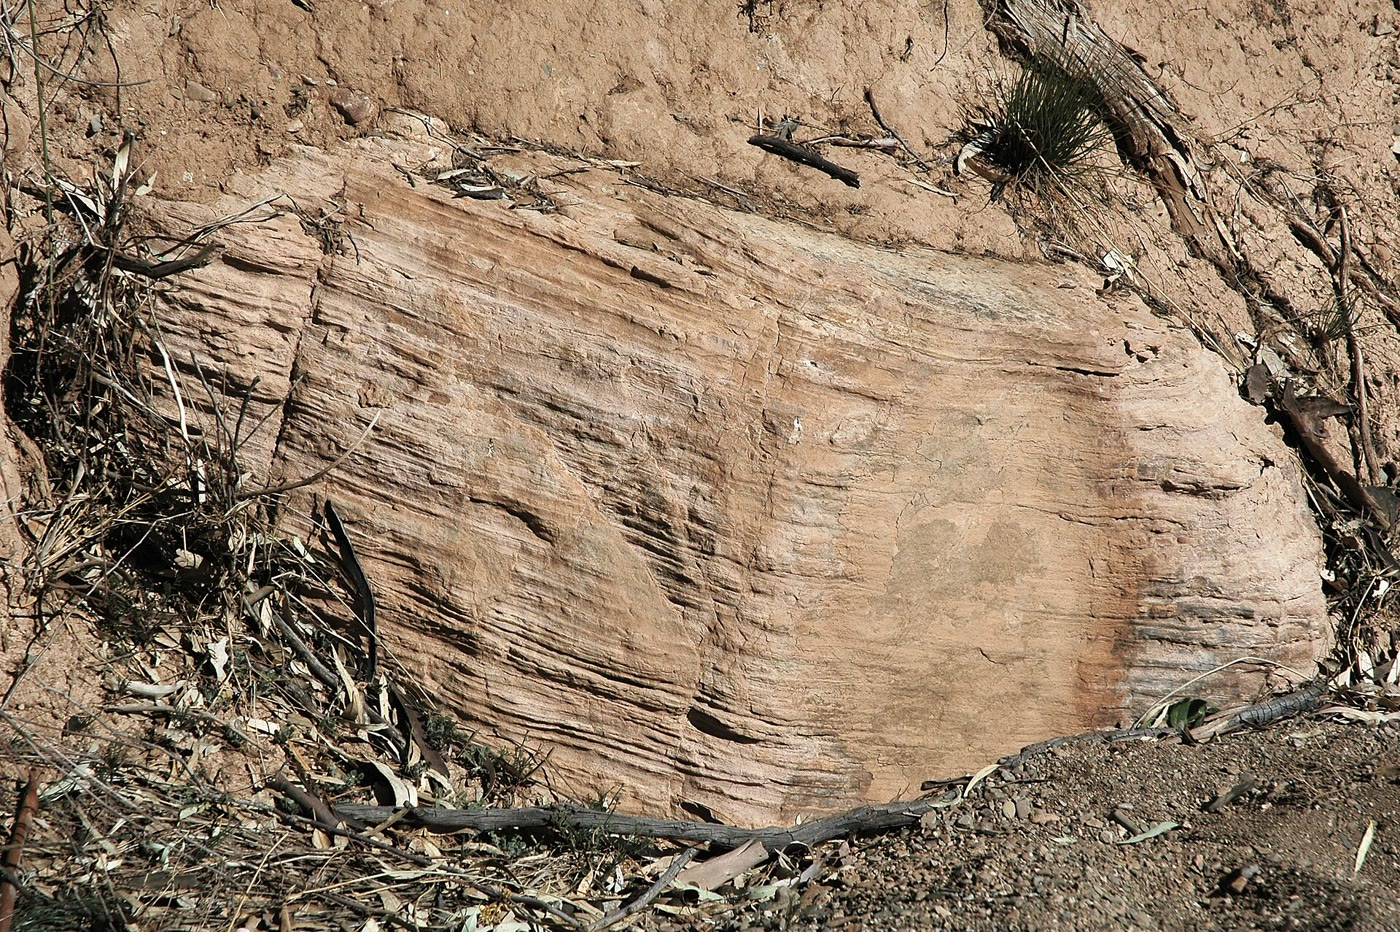
\includegraphics[width=0.66\linewidth]{images/book4/b2-18-cap-carbonate.jpg}
\par\smallskip{\small Un \omterm{def:b2:precambrian-earth:snowball}{carbonate de couverture}~: dolomie laminée de la formation de Nuccaleena,
Flinders Ranges, Australie-Méridionale, reposant sur les dépôts de la glaciation marinoenne
(les couches sont basculées). Photographie James St.~John, CC~BY~2.0 (Wikimedia Commons).}
\end{omfigure}

Deux épisodes de \omterm{def:b2:precambrian-earth:snowball}{Terre boule de neige} du Cryogénien sont aujourd'hui datés par des âges uranium--plomb sur des zircons de cendres
volcaniques et par des âges rhénium--osmium sur des schistes riches en matière organique. Le Sturtien commence entre 717.5 et
\qty{716.3}{Ma} et finit entre 659.3 et \qty{658.5}{Ma}~: \qty{58}{Ma} de glace, avec un début et une fin synchrones
dans le monde entier. Le Marinoen commence entre 649.9 et
\qty{639.0}{Ma}, datation approximative, et finit entre 636.0 et \qty{634.7}{Ma}~: au moins
\qty{3}{Ma}. Chacune se termine par un seul \omterm{def:b2:precambrian-earth:snowball}{carbonate de couverture}, jamais par plusieurs. Les formations de fer,
absentes pendant un milliard d'années, reviennent dans les dépôts glaciaires sturtiens. Au moins une boule de neige antérieure,
au sidérien vers \qty{2.4}{Ga}, a coïncidé avec la GOE~; entre les deux épisodes, pendant environ \qty{1.5}{Ga}, on ne connaît
presque aucune calotte glaciaire n'est connue.
% ledger: hoffman17:ages, hoffman17:cryochrons, hoffman17:cap, hoffman17:models, hoffman17:earlier

\begin{history}[D'une hypothèse curieuse à une théorie datée]
En 1964, W.~B. Harland attira l'attention sur les indices d'une glaciation tardive du Précambrien. En
1968 et 1969, M.~I. Budyko, puis W.~D. Sellers avec un modèle semblable, établirent que la \omterm{def:b2:precambrian-earth:ice-albedo}{rétroaction glace--albédo}
pouvait faire s'étendre la glace jusqu'à l'équateur une fois qu'elle avait assez progressé~; une Terre
globalement gelée apparut alors comme un état sans retour, et donc jamais survenu.
En 1981, J.~Walker, P.~Hays et J.~Kasting décrivirent le thermostat de l'altération des silicates et
remarquèrent que, sur une Terre gelée, le dioxyde de carbone des volcans s'accumulerait jusqu'à ce que la glace
fonde~: l'état pouvait ainsi prendre fin de lui-même. En 1992, J.~L. Kirschvink proposa qu'il se soit effectivement
produit, et le nomma «~\omterm{def:b2:precambrian-earth:snowball}{Terre boule de neige}~»~; en 1998, P.~F. Hoffman et ses collègues publièrent
«~A Neoproterozoic Snowball Earth~», et les époques panglaciaires furent appelées cryochrones. Aucun dépôt glaciaire
du Cryogénien n'avait été daté radiométriquement avant 2004~; les datations ci-dessus sont l'œuvre des années
écoulées depuis.
\end{history}
% ledger: hoffman17:history

Les volcans sont la voie de sortie. Sur une Terre couverte de glace, la pluie et les fleuves s'arrêtent presque, et avec eux
l'altération des silicates~; le dioxyde de carbone rejeté par les volcans s'accumule dans l'air
jusqu'à ce que son effet de serre fasse fondre la glace.

\begin{proposition}[Accumulation du dioxyde de carbone]\label{prop:b2:precambrian-earth:co2}
Si du dioxyde de carbone est rejeté à un débit $F$ (masse par an) dans une atmosphère de masse
$M_{\text{a}}$ et de masse molaire moyenne $\bar M$, sans puits, le temps nécessaire pour porter son rapport de
mélange volumique de presque zéro à $x$ est
\[
  \tau = \frac{x}{1 - x}\,\frac{M_{\mathrm{CO_2}}}{\bar M}\,\frac{M_{\text{a}}}{F} .
\]
\end{proposition}

\begin{proof}
L'atmosphère contient $n = M_{\text{a}}/\bar M$ moles d'autres gaz. En ajoutant $n_c$ moles de
dioxyde de carbone, son rapport de mélange vaut $x = n_c/(n + n_c)$, donc $n_c = n\,x/(1 - x)$, soit une masse de
$n_c M_{\mathrm{CO_2}}$~; au débit $F$, cela prend $\tau = n_c M_{\mathrm{CO_2}}/F$.
\end{proof}

\begin{example}[Combien de temps pour s'en sortir~?]\label{ex:b2:precambrian-earth:escape}
La meilleure estimation retenue du rejet volcanique actuel est de \qty{0.26}{Gt} de dioxyde de carbone par
an. Les estimations du rapport de
mélange nécessaire pour mettre fin à une boule de neige cryogénienne vont de 0.01 à 0.1. Avec $M_{\text{a}} =
\qty{5.1e18}{kg}$, $\bar M = \qty{28.97}{g.mol^{-1}}$ et $M_{\mathrm{CO_2}} =
\qty{44.01}{g.mol^{-1}}$, pour $x = 0.01$, il faut $\frac{0.01}{0.99}\times1.519\times\qty{5.1e18}{kg}
/ \qty{0.26e12}{kg.an^{-1}} = \qty{0.30}{Ma}$, et, pour $x = 0.1$, il faut \qty{3.3}{Ma}.
\end{example}
% ledger: usgs:volcanic-co2, hoffman17:co2, earth:Matm, earth:Mmol, ciaaw:abridged-2024
% values: co2_t001_Myr 0.301, co2_t01_Myr 3.311 (precambrian.py)

Une colonne de dioxyde de carbone pur pesant \qty{1}{bar} sur toute la Terre demanderait
\qty{20}{Ma} au même débit, le chiffre donné par Walker, Hays et Kasting. Quelques millions d'années
est long, mais le Sturtien a duré \qty{58}{Ma}. Ou bien le seuil était plus élevé, ou bien le
dégazage plus faible, ou bien la Terre gelée avait encore des puits~: l'altération du plancher océanique jeune,
qui ne s'arrête pas sous la glace, en est un candidat. Dans le modèle de bilan d'énergie, la sortie exige que l'émissivité effective
de la boule de neige baisse jusqu'à ce que sa température atteigne \qty{263}{K}~: sous le Soleil du Cryogénien,
\qty{94}{\percent} de l'actuel, de 0.616 à 0.472, soit un piégeage supplémentaire d'environ
\qty{39}{W.m^{-2}} (\cref{exo:b2:precambrian-earth:10}).
% ledger: hoffman17:co2, hoffman17:models, usgs:volcanic-co2
% values: one_bar_Myr 19.98, eps_melt_094 0.4716, forcing_melt_094 39.1 (precambrian.py)

Lorsque la glace s'ouvre enfin à l'équateur, la rétroaction joue en sens inverse~: la mer sombre absorbe davantage
de rayonnement solaire, la glace recule, et les modèles font courir la ligne de glace vers les pôles en
environ \qty{2}{ka}. La Terre se retrouve alors avec un effet de serre énorme sur une surface sombre, une
phase chaude qui suit. L'altération, très rapide dans ce climat, déverse calcium, magnésium et bicarbonate dans
la mer, où les \omterm{def:b2:precambrian-earth:snowball}{carbonates de couverture} précipitent tandis que l'eau de fonte inonde les plateaux continentaux~; il faut
une dizaine de millions d'années pour faire redescendre le dioxyde de carbone. Les calottes glaciaires et les \omterm{def:b2:precambrian-earth:snowball}{carbonates
de couverture}, les formations de fer et la synchronie des âges expliquent pourquoi la plupart des géologues admettent
aujourd'hui que les boules de neige du Cryogénien ont bien eu lieu, bien que leur intensité --- savoir si une ceinture
d'eau libre a survécu à l'équateur, comme le proposent les modèles de «~ceinture d'eau~» --- reste discutée.
% ledger: hoffman17:hysteresis, hoffman17:cap, hoffman17:debate

\section*{Exercices}\label{sec:b2:precambrian-earth:exercises}

Données~: sauf indication contraire, $\sigma = \qty{5.670e-8}{W.m^{-2}.K^{-4}}$~;
$S_0 = \qty{1361}{W.m^{-2}}$~; albédo actuel 0.294 et température moyenne de surface \qty{288}{K}~;
albédo de la boule de neige 0.6~; rampe de \qty{263}{K} à \qty{283}{K}~; émissivité effective actuelle
0.616~; loi de Gough $L/L_0 = 1/(1 + 0.4\,t/t_\odot)$ pour un temps $t$ avant le présent, $t_\odot =
\qty{4.567}{Ga}$~; liquidus de \omterm{def:b2:precambrian-earth:greenstone}{komatiite} \qty{1616}{\celsius} à \qty{32.2}{\percent} de MgO,
pente \qty{18.0}{\celsius} par point de pourcentage~; demi-vies \ce{^{238}U} \qty{4.468}{Ga}, \ce{^{235}U}
\qty{0.704}{Ga}, \ce{^{232}Th} \qty{14.0}{Ga}, \ce{^{40}K} \qty{1.248}{Ga}.
% ledger: const:sigma, earth:TSI, earth:albedo, earth:Tsurf, hoffman17:models, gough81:luminosity, connelly12:cai, so16:liquidus, iaea:isotopes

\begin{exercise}[$\star$]\label{exo:b2:precambrian-earth:1}
(a) Combien de temps ont duré l'\omterm{def:b2:precambrian-earth:eons}{Hadéen}, l'\omterm{def:b2:precambrian-earth:eons}{Archéen} et le \omterm{def:b2:precambrian-earth:eons}{Protérozoïque}~? (b) Quelle fraction de l'âge
de la Terre représentent ensemble les trois~? (c) Quel âge avait la Terre quand le plus ancien zircon connu a cristallisé,
et quand se sont formées les roches les plus anciennes~?
\end{exercise}

\begin{exercise}[$\star$]\label{exo:b2:precambrian-earth:2}
Aujourd'hui, la \omterm{def:b2:elements-in-the-earth:bse}{Terre silicatée globale} libère, par kilogramme, \qty{1.917}{pW} venant de \ce{^{238}U},
\qty{0.082}{pW} venant de \ce{^{235}U}, \qty{2.089}{pW} de \ce{^{232}Th} et \qty{0.818}{pW} de
\ce{^{40}K} ($\qty{1}{pW} = \qty{e-12}{W}$). (a) Calculer chaque contribution il y a \qty{3}{Ga}, et
le total. (b) De quel facteur la production de chaleur a-t-elle diminué depuis~? (c) Quel isotope domine
aujourd'hui, et lequel dominait alors~?
\end{exercise}

\begin{exercise}[$\star$]\label{exo:b2:precambrian-earth:3}
Utiliser le thermomètre à \omterm{def:b2:precambrian-earth:greenstone}{komatiites}. (a) Quel est le liquidus d'une \omterm{def:b2:precambrian-earth:greenstone}{komatiite} à
\qty{28}{\percent} de MgO~? (b) Quelle teneur en MgO correspond à \qty{1500}{\celsius}~? (c) Une
coulée à texture spinifex a une teneur en MgO de roche totale de \qty{38}{\percent}.
Pourquoi son liquidus ne doit-il pas être lu sur la droite~?
\end{exercise}

\begin{exercise}[$\star$]\label{exo:b2:precambrian-earth:4}
Mettre dans l'ordre les événements suivants et donner leurs âges approximatifs~: la \omterm{def:b2:precambrian-earth:goe}{Grande Oxydation}, les
premiers stromatolithes, la fin de la glaciation marinoenne, les dernières \omterm{def:b2:precambrian-earth:greenstone}{komatiites} courantes, les
roches les plus anciennes, la seconde montée de l'oxygène, les premiers fossiles édiacariens, la fin des
structures dômes-et-quilles de la Pilbara.
\end{exercise}

\begin{exercise}[$\star\star$]\label{exo:b2:precambrian-earth:5}
(a) Vérifier que l'émissivité effective de la Terre actuelle vaut 0.616. (b) Trouver l'équilibre de la boule de neige
sous le Soleil actuel. (c) Montrer que l'équilibre intermédiaire, \qty{275.5}{K}, vérifie
$R = E$ à \qty{0.5}{W.m^{-2}} près. (d) Trouver les pentes de $R$ et de $E$ en ce point, et conclure
qu'il est instable.
\end{exercise}

\begin{exercise}[$\star\star$]\label{exo:b2:precambrian-earth:6}
(a) En utilisant la loi de Gough, trouver le rayonnement solaire il y a \qty{2.4}{Ga} et il y a \qty{0.65}{Ga}, en fractions
de l'actuel. (b) Dans le modèle, un climat chaud est-il possible à chaque date avec l'émissivité actuelle~?
(c) Hoffman et ses collègues écrivent que le Soleil sidérien était environ \qty{10}{\percent} moins brillant que le
Soleil du Cryogénien. Vérifier.
\end{exercise}

\begin{exercise}[$\star\star$]\label{exo:b2:precambrian-earth:7}
Le Sturtien a duré de \qty{716.9}{Ma} à \qty{658.9}{Ma} (milieux des intervalles datés),
le Marinoen de \qty{644.5}{Ma} à \qty{635.4}{Ma}. (a) Calculer leurs durées, ainsi que
l'interglaciaire qui les sépare. (b) Quelle fraction de la période du Cryogénien, de 720 à \qty{635}{Ma},
la glace a-t-elle couvert la Terre, selon ces chiffres~? (c) Pourquoi la durée du Marinoen n'est-elle qu'un
ordre de grandeur~?
\end{exercise}

\begin{exercise}[$\star\star$]\label{exo:b2:precambrian-earth:8}
(a) Combien de temps faut-il aux volcans, à \qty{0.26}{Gt} par an sans puits, pour porter l'air à un
rapport de mélange du dioxyde de carbone de 0.05~? (b) Combien de fois les \qty{278}{ppm} de 1750 cela fait-il~? (c) Si la moitié
du rejet était captée par l'altération du plancher océanique, combien de temps faudrait-il~?
\end{exercise}
% ledger: usgs:volcanic-co2, earth:Matm, earth:Mmol, ciaaw:abridged-2024, ipcc:erf-2xco2

\begin{exercise}[$\star\star$]\label{exo:b2:precambrian-earth:9}
Un dépôt diamictitique néoprotérozoïque contient des pierres striées, dont certaines reposent dans une boue finement laminée
qui se courbe sous elles. (a) Qu'indique cette courbure~? (b) Sa paléolatitude est
\ang{10}. Pourquoi cela compte-t-il pour l'hypothèse de la boule de neige~? (c) Elle est directement recouverte d'une
dolomie rose laminée de quelques mètres d'épaisseur. De quoi s'agit-il, et qu'enregistre-t-elle~?
\end{exercise}

\begin{exercise}[$\star\star\star$]\label{exo:b2:precambrian-earth:10}
Sous le Soleil du Cryogénien, $S = 0.94\,S_0$. (a) Montrer que, dans le modèle, l'état chaud subsiste encore,
tout juste, mais qu'une boule de neige existe aussi. (b) Trouver la température de la boule de neige avec
l'émissivité actuelle. (c) Trouver l'émissivité à laquelle la boule de neige atteint \qty{263}{K} et dégèle. (d) Convertir
la variation d'émissivité en un piégeage supplémentaire du rayonnement infrarouge à
\qty{263}{K}, en \unit{W.m^{-2}}.
\end{exercise}

\begin{exercise}[$\star\star\star$]\label{exo:b2:precambrian-earth:11}
(a) En utilisant les points de bascule de la \cref{prop:b2:precambrian-earth:tipping}, montrer que la largeur
de la boucle d'hystérésis, $S_{\text{m}}/S_{\text{f}}$, ne dépend pas de l'émissivité, et la calculer. (b) Qu'est-ce qui
rendrait la boucle plus étroite~? (c) Pourquoi une boule de neige ne peut-elle dégeler que loin des
conditions dans lesquelles elle a gelé~?
\end{exercise}

\begin{exercise}[$\star\star\star$]\label{exo:b2:precambrian-earth:12}
Établir la constante de temps du modèle de bilan d'énergie près de l'équilibre chaud, $\tau =
C/(E'(T^*) - R'(T^*))$, et l'évaluer pour une couche de mélange océanique de \qty{50}{m} de profondeur, de masse volumique
\qty{1025}{kg.m^{-3}} et de chaleur massique \qty{3992}{J.kg^{-1}.K^{-1}}. Que devient $\tau$ lorsque le
rayonnement solaire approche du point de bascule de gauche, dans ce modèle et dans un modèle dont l'albédo varie
continûment avec la température~?
\end{exercise}
% ledger: noaa:seawater-1025, teos10:cp0

\begin{problem}[{Problème du week-end --- Une jeune Terre plus chaude}]\label{pb:b2:precambrian-earth:1}
Ce problème suit la jeune Terre de son intérieur à son air. Utiliser les données des
exercices~; la \omterm{def:b2:elements-in-the-earth:bse}{Terre silicatée globale} contient \qty{0.0203}{ppm} d'uranium, \qty{0.0795}{ppm} de
thorium et \qty{240}{ppm} de potassium en masse, et ses isotopes libèrent \qty{95.13}{\micro W}
(\ce{^{238}U}), \qty{568.47}{\micro W} (\ce{^{235}U}), \qty{26.28}{\micro W} (\ce{^{232}Th}) et
\qty{28.47}{\micro W} (\ce{^{40}K}) par kilogramme d'isotope. En masse, l'uranium est
à \qty{99.29}{\percent} de \ce{^{238}U} et à \qty{0.711}{\percent} de \ce{^{235}U}, et le potassium
à \qty{0.0120}{\percent} de \ce{^{40}K}. Arrondir à trois chiffres significatifs.

\noindent\textbf{Partie I --- Chaleur venue de l'intérieur.}
\begin{enumerate}
  \item Trouver la chaleur libérée aujourd'hui par chaque isotope par kilogramme de \omterm{def:b2:elements-in-the-earth:bse}{Terre silicatée globale}, en
        \unit{pW.kg^{-1}}.
  \item Trouver le total.
  \item Trouver la constante de désintégration de chaque isotope, en \unit{Ga^{-1}}.
  \item Trouver chaque contribution il y a \qty{2.7}{Ga}, lorsque les \omterm{def:b2:precambrian-earth:greenstone}{komatiites} de Pyke Hill ont fait éruption.
  \item Trouver le total alors, et le rapport à celui d'aujourd'hui.
  \item Quel isotope dégageait le plus de chaleur alors~? Pourquoi en dégage-t-il si peu aujourd'hui~?
\end{enumerate}

\noindent\textbf{Partie II --- Le Soleil de l'Archéen.}
\begin{enumerate}[resume]
  \item Avec la loi de Gough, trouver le rayonnement solaire il y a \qty{2.7}{Ga} en fraction de l'actuel, et en
        \unit{W.m^{-2}}.
  \item Trouver l'équilibre chaud sous ce rayonnement solaire avec l'émissivité actuelle. Est-ce un état chaud
        valide du modèle~?
  \item Trouver l'équilibre de la boule de neige sous ce rayonnement solaire.
  \item Quelle émissivité effective maintiendrait la Terre à \qty{288}{K} avec l'albédo chaud~?
  \item Le dioxyde de carbone seul aurait pu le faire à 0.004 à \qty{0.03}{bar} à \qty{2.5}{Ga}.
        Dans une atmosphère d'environ \qty{1}{bar}, combien de fois les \qty{278}{ppm} de 1750 cela
        fait-il~?
  \item Nommer le processus qui a maintenu le dioxyde de carbone à un tel niveau pendant des centaines de millions
        d'années.
\end{enumerate}

\noindent\textbf{Partie III --- Une boule de neige et sa fin.}
\begin{enumerate}[resume]
  \item La première boule de neige, il y a \qty{2.4}{Ga}~: trouver le rayonnement solaire d'alors en fraction de l'actuel.
        L'état chaud du modèle est-il encore possible avec l'émissivité actuelle~?
  \item Avec \qty{0.26}{Gt} de dioxyde de carbone par an, combien de temps faut-il pour atteindre un rapport de
        mélange de 0.1~?
  \item Si le seuil sous le Soleil sidérien, moins brillant, était deux fois plus élevé, 0.2, combien de temps faudrait-il~?
  \item Quelle roche enregistre la fin d'une boule de neige, et comment~?
  \item Pourquoi les formations de fer du Sturtien ont-elles besoin d'un océan sans oxygène sous la glace~?
\end{enumerate}

\noindent\textbf{Partie IV --- Le thermomètre à komatiites.}
\begin{enumerate}[resume]
  \item Vérifier la pente de la droite des \omterm{def:b2:precambrian-earth:greenstone}{komatiites} à partir des deux expériences.
  \item Un liquide de \omterm{def:b2:precambrian-earth:greenstone}{komatiite} de Pyke Hill contenait \qty{30}{\percent} de MgO. Trouver son liquidus.
  \item Trouver le liquidus de la \omterm{def:b2:precambrian-earth:greenstone}{komatiite} de Barberton, à \qty{32.2}{\percent} de MgO.
  \item Trouver le liquidus d'un basalte primaire de dorsale à \qty{12}{\percent} de MgO.
  \item Avec la pente du Kilauea, \qty{20}{\celsius} par point de pourcentage, plutôt, quelle serait la température du
        basalte en partant du point de Barberton~? Quelle importance a le choix de la pente~?
  \item Pourquoi l'écart de température entre les deux laves est-il plus grand que l'écart de température
        potentielle entre le manteau archéen et le manteau actuel~?
  \item En résumé, de combien la lave de \omterm{def:b2:precambrian-earth:greenstone}{komatiite} archéenne la plus chaude était-elle plus chaude qu'un basalte primaire
        des dorsales actuelles~?
\end{enumerate}
\end{problem}
% ledger: ms95:pm-trace, dye:isotope-heat, iaea:isotopes, gough81:luminosity, cz20:archean-air, ipcc:erf-2xco2, usgs:volcanic-co2, hoffman17:co2, so16:liquidus, helz98:glass-thermometer, pierru22:komatiite
